\textbf{See the instruction for questions \inteval{\value{question}+1} to \inteval{\value{question}+2}.}

\begin{center}
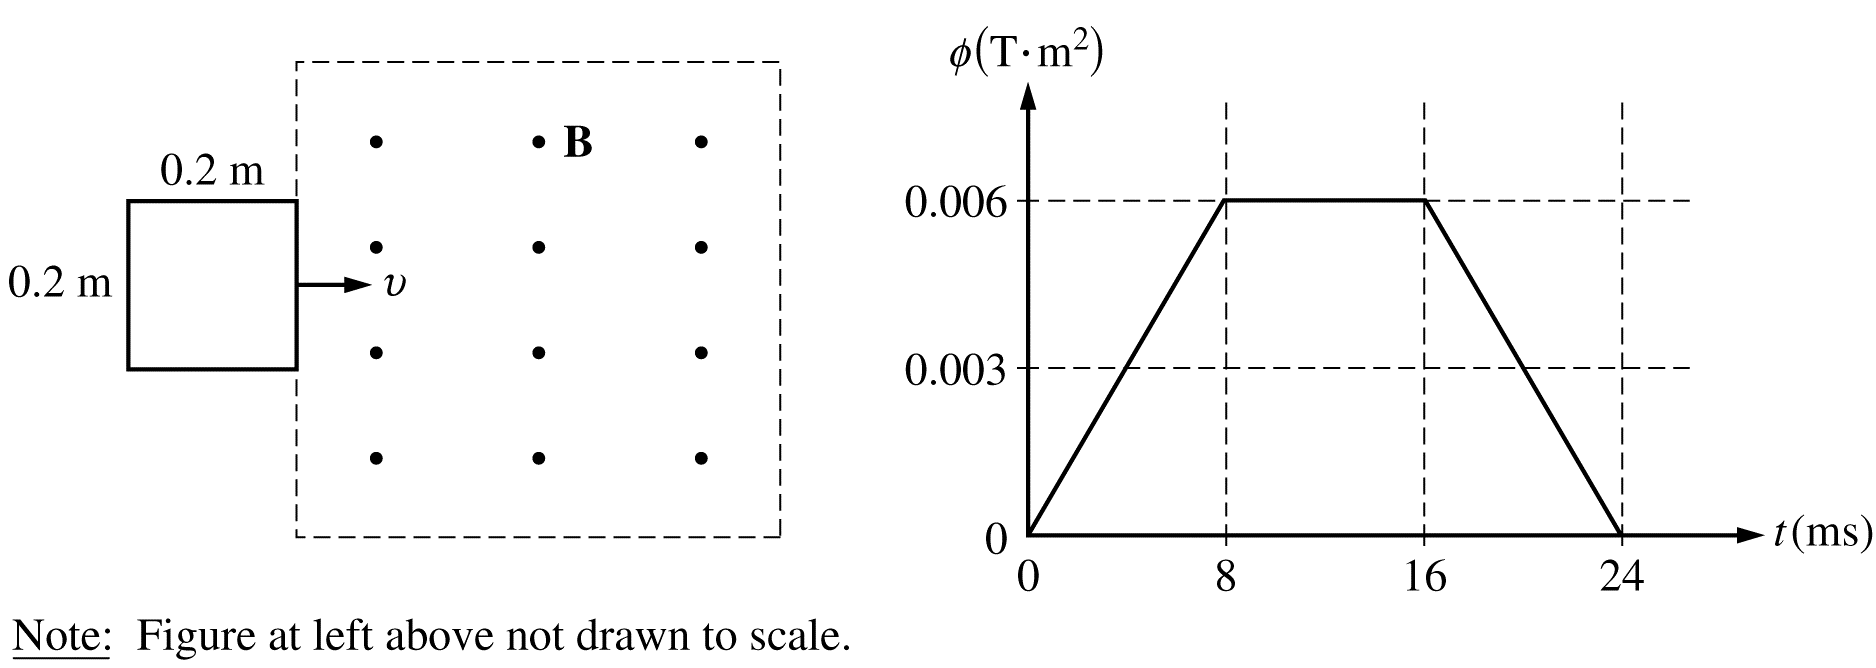
\includegraphics[scale=0.25]{images/img-006-006.png}
\end{center}

A square wire loop of side $0.2 \unit{m}$ moves with a constant speed of $v=25 \unit{m/s}$ through a region containing a magnetic field of strength $B=0.15 \unit{T}$, as shown above left. A graph of the magnetic flux $\phi$ through the loop as a function of time $t$ is shown above right. Time $t=0$ occurs when the right edge of the loop just begins to enter the field.

% Multiple Choice Question 9
\begin{questions}\setcounter{question}{8}\question
What is the magnitude of the induced emf in the wire loop at $t=4 \unit{ms}$ ?

\begin{oneparchoices}
\choice $0 \unit{V}$
\choice $0.50 \unit{V}$
\choice $0.75 \unit{V}$
\choice $3.0 \unit{V}$
\choice $6.0 \unit{V}$
\end{oneparchoices}\end{questions}

% Multiple Choice Question 10
\begin{questions}\setcounter{question}{9}\question
What is the total width of the magnetic field through which the loop moves?

\begin{oneparchoices}
\choice $0.1 \unit{m}$
\choice $0.2 \unit{m}$
\choice $0.4 \unit{m}$
\choice $0.6 \unit{m}$
\choice $0.8 \unit{m}$
\end{oneparchoices}\end{questions}

